\section{Proposed hybrid method}\label{proposed-hybrid-method}

A hybrid method is proposed in this section, where wave damping $B_W$
(including the speed dependent wave damping) obtained implicitly with
FNPF is used together with the viscous damping contributions from
Ikeda's method. The viscous damping is added to the FNPF simulations by
injecting the viscous parts of the linear and quadratic damping
coefficients (obtained with Ikeda's method) to the equation of motion.

Ikeda's method divides roll damping into five damping components:

\begin{longtable}[]{@{}ll@{}}
\toprule
Symbol & Component\tabularnewline
\midrule
\endhead
$B_F$ & skin friction\tabularnewline
$B_E$ & eddy generation\tabularnewline
$B_L$ & hull lift\tabularnewline
$B_W$ & roll wave generation\tabularnewline
$B_{BK}$ & bilge keels\tabularnewline
\bottomrule
\end{longtable}

The total damping is calculated as the sum of these components
\cite{7505983/937PN5DT},

\begin{equation}
B = B_F + B_E + B_L + B_W + B_{BK}
\end{equation}

Ikeda has in a series of papers proposed semi empirical formulas for the
viscous damping components: $B_F$, $B_E$, $B_{BK}$ and $B_L$ so
that viscous damping can be obtained from,

\begin{equation}
\label{eq:viscous damping}
B_{visc} = B_F + B_E + B_L
\end{equation}

In order to reduce the number of uncertain parameters, the bilge keel
damping $B_{BK}$ has been exluded above, thereby assuming that the
ship does not have bilge keels.

Ikeda produced many papers about various aspects of roll damping where
most of them are translations from original manuscripts written in
Japanese. Summaries of this method \cite{7505983/FB64RGPF},
\cite{7505983/KAKIM2E2} and \cite{7505983/UGK6YEVD} has been used
together with the original papers to understand how the method should be
implemented. Falzarano says that the Himeno report and associated
computer programs are well-known to have numerous typographical errors.
When looking at these resources it becomes evident that there is some
variety on how the method should be implemented, regardless if this is
due to typographical errors or being variations of the actual method.
The implementation was therefore a fairly time consuming task where
various alternative implementations needed to be compared and
investigated.

The scale effects of roll damping is considered to mainly be associated
with the skin friction component $B_F$ \cite{7505983/FB64RGPF}. This
component constitute a very small part of the total damping for the full
scale ship, but a substantial part for the model scale ship used in this
study. This is therefore the only component in Ikedas method that needs
to be recalculated when the scale changes.

For the skin friction damping $B_F$ implementation was made according
to the description in \cite{7505983/UGK6YEVD}. With the difference that
the actual wetted surface at rest $S$ was used instead of the proposed
estimation formula.

The hull lift damping $B_L$ is calculated according to
\cite{7505983/937PN5DT} and implemented as described in
\cite{7505983/UYUAYY7E}. Journ\'ee added a linear interpolation to the
values for $\kappa$ from the Ikeda's paper.

Ikeda's method calculates the roll damping at a certain roll angle
frequency $\omega$ and roll angle amplitude $\phi_a$. A schematic
graph of how the parameters vary with speed and roll angle amplitude
$\phi_a$ is shown in fig.\ref{fig:ikeda_generic}. The roll
amplitude is first varied at zero speed (left). The speed is then varied
from zero to the froude number corresponding to 15.5 knots in full scale
for the KVLCC2 with a roll angle amplitude of 10 degrees (middle). The
amplitude is then gradually reduced at the highest froude number down to
zero again (right).

Assumming that the trends are correct in Ikeda's method it can be noted
from the amplitude variations at zero knots (left):

\begin{itemize}
\item $B_W$ does not change with amplitude, implying that they only contribute to the linear part ($B_1$) of the damping. (The $B_W$ was calculated with strip theory here)
\item $B_F$ has a small amplitude dependancy but the linear part is dominating.
\item $B_E$ has a large amplitude depandancy and only contributes to the quadratic damping ($B_2$)\cite{7505983/4AFVVGNT}.
\end{itemize}

Looking at the speed variation (middle):

\begin{itemize}
\item At low speed $B_F$ and $B_E$ are the dominating components. (Note that this ship does not have bilge keels, as that would otherwise also be a large component).
\item At high speed the $B_E$ has almost disappeared and is replaced by the $B_L$ which is now the dominating component.
\item $B_F$ has a large contribution for all speeds (at model scale).
\end{itemize}

Looking at the roll amplitude variation (right):

\begin{itemize}
\item (Please note that this x-axis is revered in this graph)
\item $B_L$ does not change with amplitude, implying that they only contribute to the linear part ($B_1$) of the damping.
\item $B_F$ has a small amplitude dependancy but the linear part is dominating.
\end{itemize}

    

    \begin{Verbatim}[commandchars=\\\{\}]

    \end{Verbatim}

    \begin{figure}[H]
        \begin{center}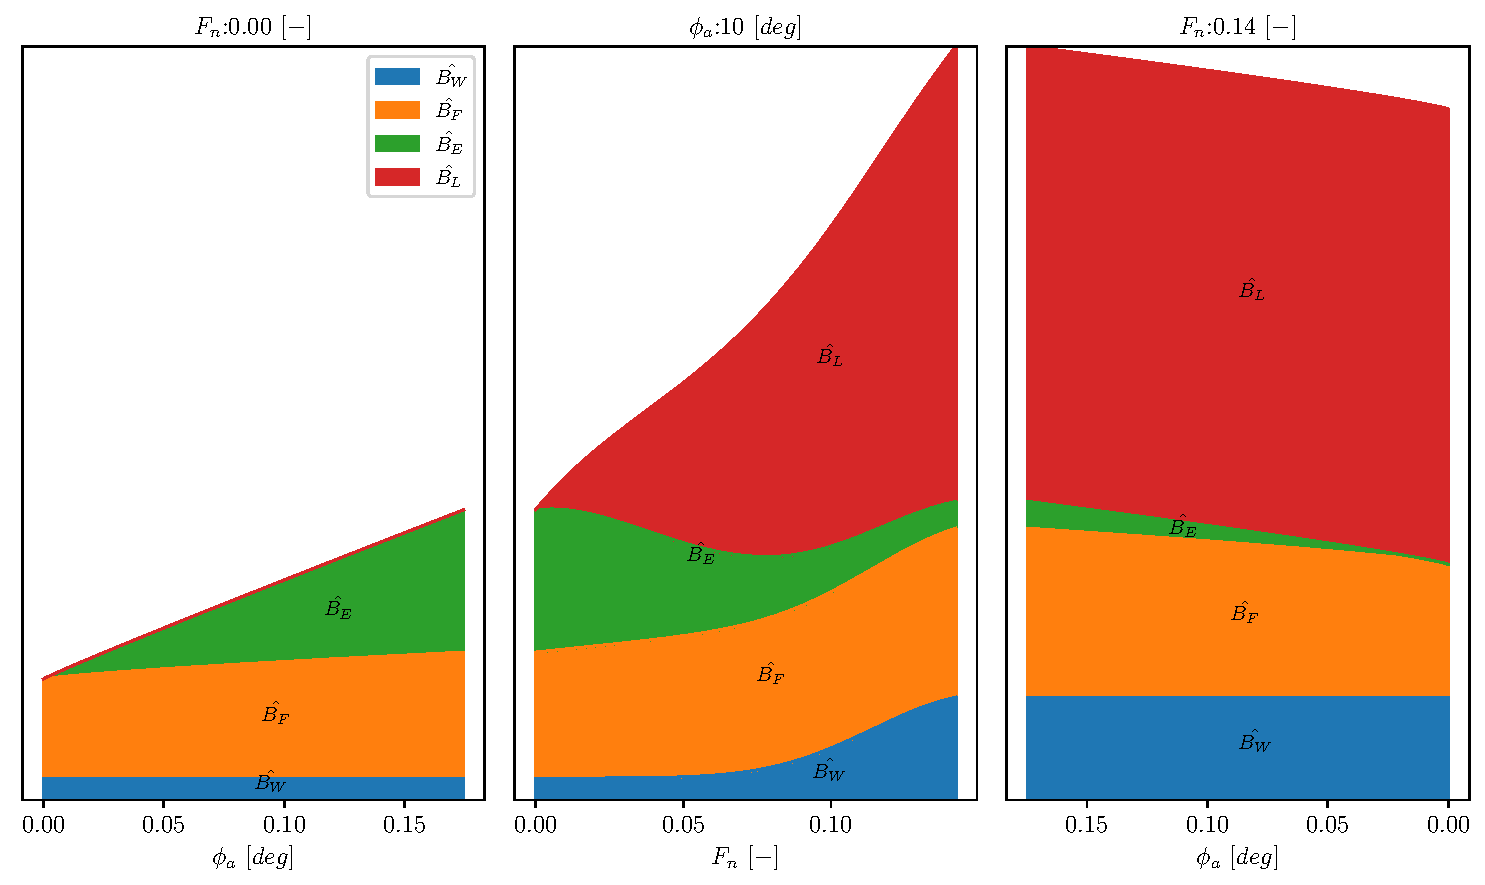
\includegraphics[width = 0.5\textwidth]{figures/ikeda_generic.pdf}\end{center}
        \vspace{-1cm}
        \caption{Ikeda generic}
        \label{fig:ikeda_generic}
    \end{figure}
    
    When the damping predicted with Ikeda's method was compared with
corresponding model test it was found that the results were in poor
agreement for the zero speed case but quite good results at speed. This
was pointing towards the eddy damping being incorrect in the current
implementation of Ikeda's method. A thorough investigation of the eddy
damping prediction was therefore conducted which is described in the
next section.

    \subsection{Eddy damping}\label{eddy-damping}

The eddy damping is due to eddies generated around the ship hull during
the roll motion. Strong eddies occures at sharp edges in the geometry.
Below is an illustration of how the eddy damping changes with bilge
radius to beam ratio as predicted with the current implementation of the
method. It seems that the damping approaches zero very fast as the bilge
radius increase. So having just a small rounding of the bilge, compared
to a square section, will have a great impact on the eddy roll damping.

    \begin{figure}[H]
        \begin{center}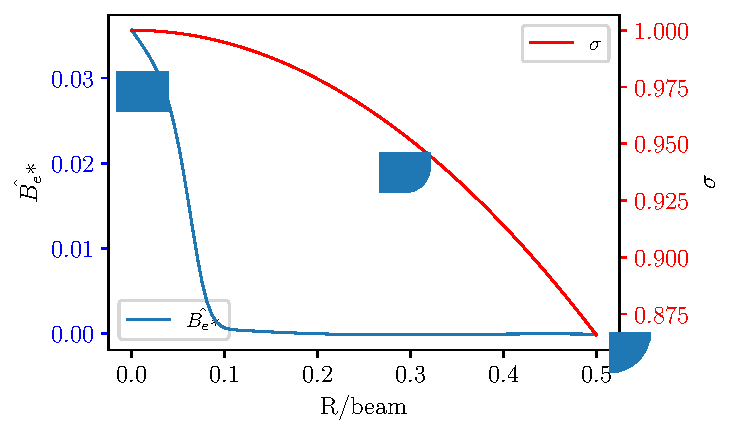
\includegraphics[width = 0.5\textwidth]{figures/eddy_sigma.pdf}\end{center}
        \vspace{-1cm}
        \caption{Eddy sigma}
        \label{fig:eddy_sigma}
    \end{figure}
    
    Ikeda made experiements on a number of two-dimensional cylinders with
various sections \cite{7505983/4AFVVGNT}. Ikeda found that the eddy
damping per unit length of these sections can be expressed as: 
 
            
    
    \begin{equation}
B'_{E0} = \frac{4 C_{r} T_{s}^{4} \omega \phi_{a} \rho}{3 \pi}
\label{eq:eddy_section}
\end{equation}

    

    The total eddy damping can be obtained as an integral over the sections
along the ship hull:
 
            
    
    \begin{equation}
B_{E0} = \int\limits_{AP}^{FP} B'_{E0}\, dx
\label{eq:equation}
\end{equation}

    

    It can be seen from the section damping (eq.
\ref{eq:eddy_section}) above that the eddy damping increases
linearly with both roll amplitude and frequency, and that it will go to
zero for small amplitudes and frequencies, which means that it is only
included in the quadratic damping term ($B_2$). Ikeda expressed the
$C_r$ coefficient to be entirely depending on the hull form. Ikeda
developed a regression formula for $C_r$ based on his experiments,
which is used in the prediction method. The authors of this paper have
tried to implement this method according to the description in the
original paper \cite{7505983/4AFVVGNT} but have failed to reproduce the
results from Ikeda's experiments exactly. Other resources such as
\cite{7505983/FB64RGPF} and \cite{7505983/KAKIM2E2} have also been used
without success.

Instead, a new regression for $C_r$ was made on the experimental
results from \cite{7505983/4AFVVGNT}. The experimental results were
collected by the authors using manual digitalization
\cite{7505983/RXYIE6UW}.

    Where $OG/d=0$ for all sections. For the Series60 sections (G-K) the
bilge radius $R_b$ was estimated using the following estimation,
proposed by the authors:
 
            
    
    \begin{equation}
R_{b} = \frac{\sqrt{B_{s} T_{s} \left(1 - \sigma\right)}}{\sqrt{1 - \frac{\pi}{4}}}
\label{eq:equation}
\end{equation}

    

    The nondimensional damping is expressed in \cite{7505983/4AFVVGNT} using
an asterisk, or star symbol (*). The reason seems to be that Ikeda
wanted to signal that this damping only has the quadratic part of the
damping. This stared damping is defined as:
 
            
    
    \begin{equation}
B_{E0 HAT} = \frac{8 B_{E star hat}}{3 \pi}
\label{eq:equation}
\end{equation}

    

    $\hat{B_E}^*$ and $(B_W+B_F)^*$ are the experimental values taken
from \cite{7505983/4AFVVGNT}. Which add up to the total damping:

    $\hat{B^*} = \hat{B^*_E} + (B_W+B_F)^*$
 
            
    
    \begin{equation}
B_{E0 HAT} = \frac{8 B_{E star hat}}{3 \pi}
\label{eq:equation}
\end{equation}

    

    And the $C_r$ was calculated from the experiments as:
 
            
    
    \begin{equation}
C_{r} = \frac{3 \pi B_{E0 HAT} B_{s} T_{s} beam^{2} \sigma}{4 T^{4} \omega_{hat} \phi_{a}}
\label{eq:equation}
\end{equation}

    

    Instead of trying to invent a complicated mathematical expression for
the $C_r$ regression a simple decision tree model was instead fitted
to the $C_r$ data from Ikeda's experiments. The fitted decision tree
is illustrated in the figure below:

    \begin{figure}[H]
        \begin{center}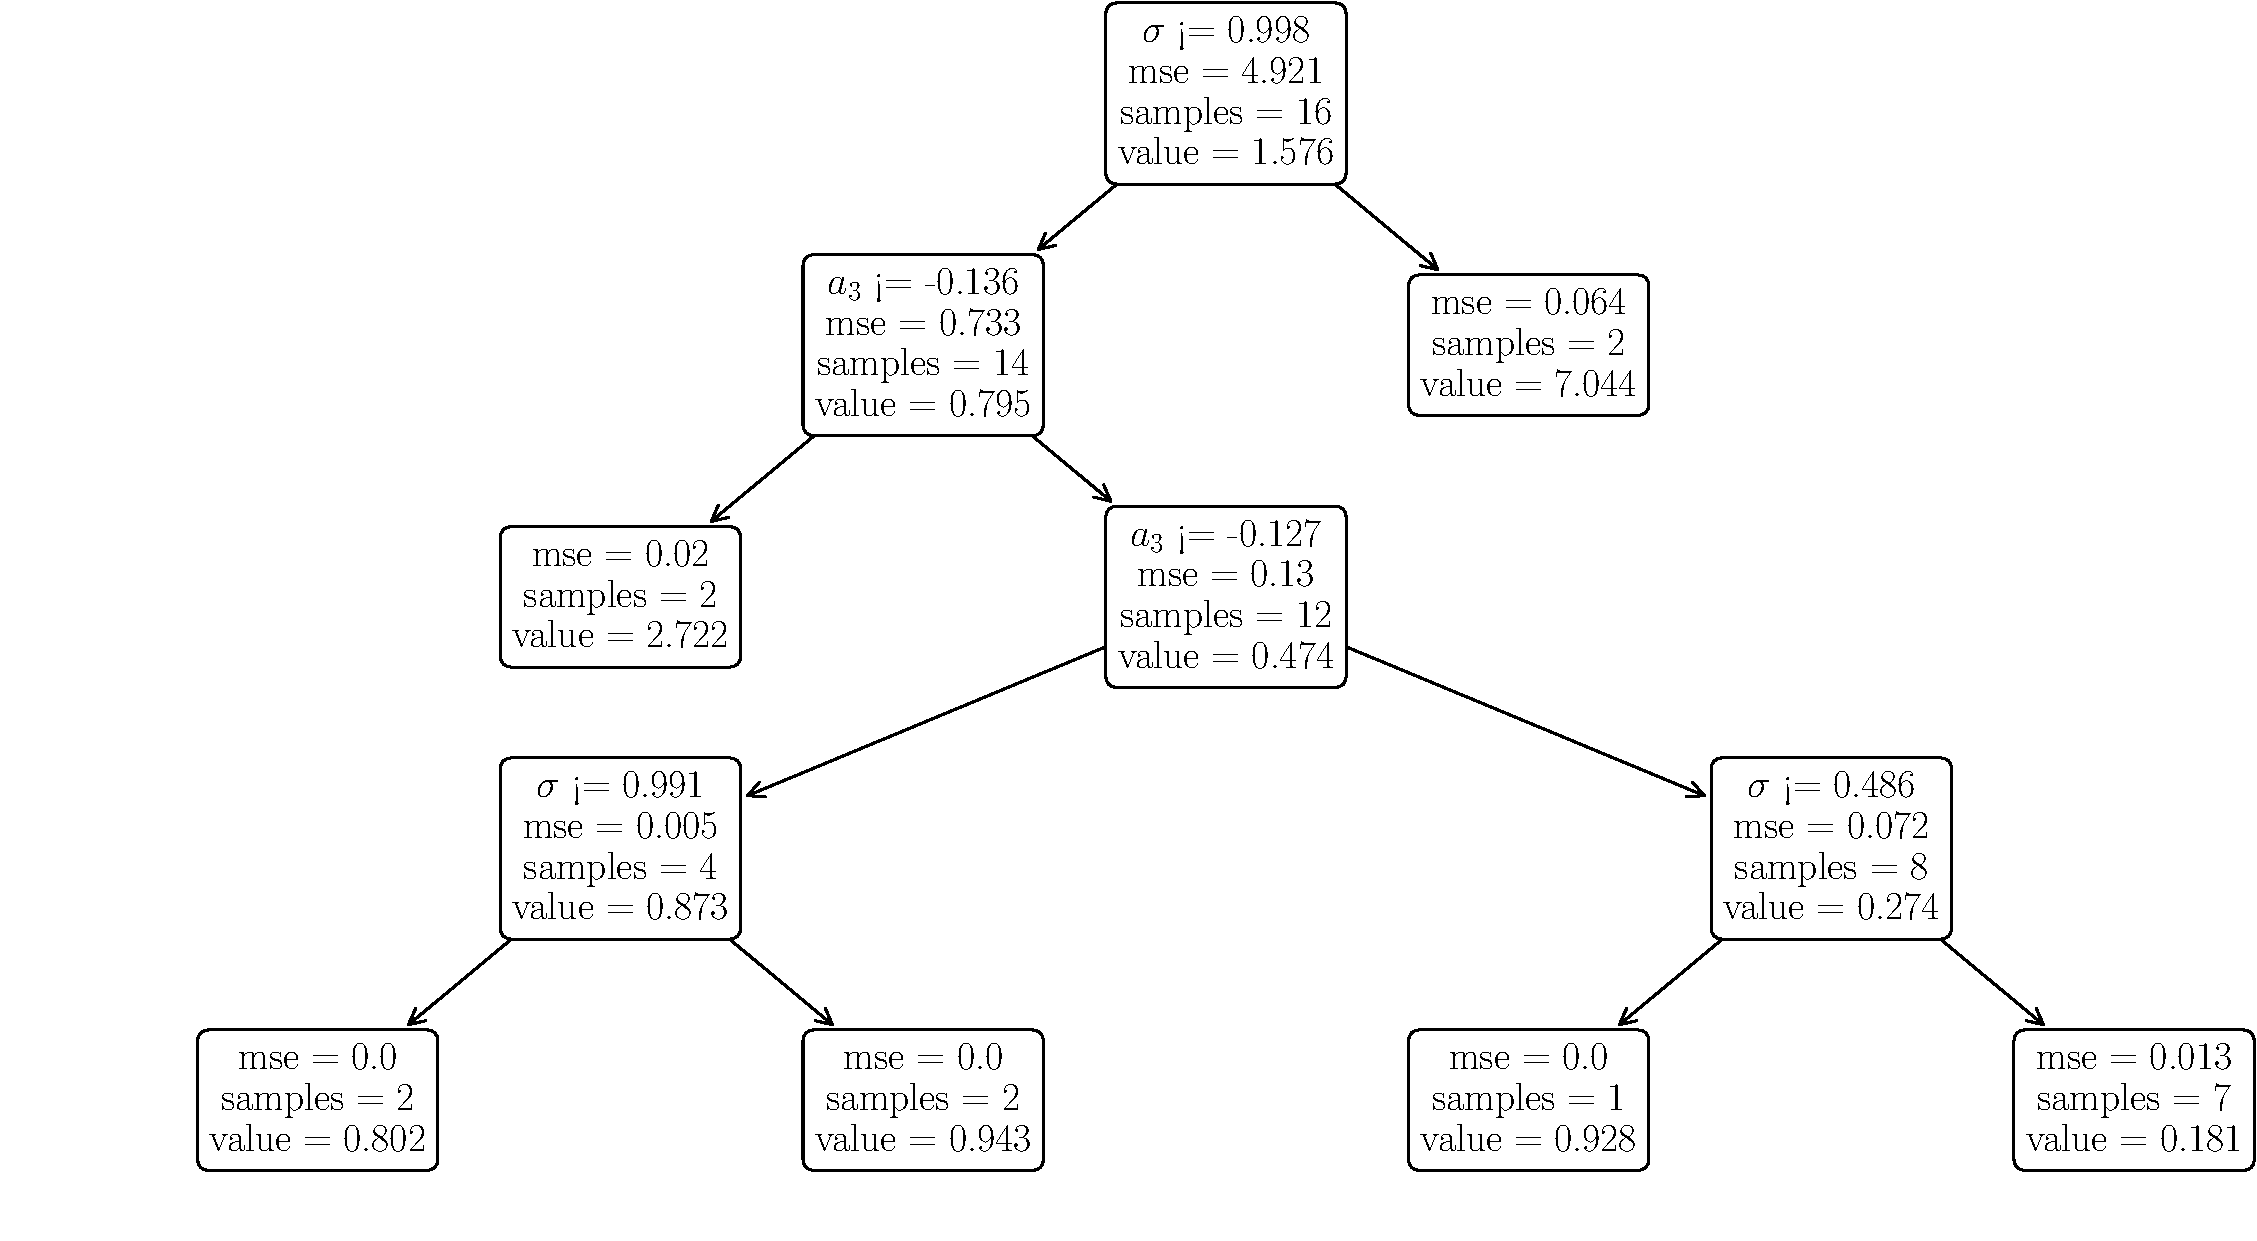
\includegraphics[width = 0.5\textwidth]{figures/decision_tree.pdf}\end{center}
        \vspace{-1cm}
        \caption{Decision tree}
        \label{fig:decision_tree}
    \end{figure}
    
    Even thoug this tree is very simple it has very good accuracy in
reproducing the results from Ikedas experiments ($r^2=0.996)$.

    \subsection{FNPF method}\label{fnpf-method}

\label{fnpf-method} Wave damping was obtained using PIT on roll decay
simulation using the fully nonlinear potential flow method. This method
is characterized by the application of the complete dynamic and
kinematic free surface boundary conditions on the instantaneous free
surface as well as the body-exact approach where the instantaneous
wetted body surface is considered in the boundary value problem for the
velocity potential, i.e. no linearizations are made to the governing
equations of the potential flow problem.

The method used in this study employs a boundary element method (BEM)
\cite{7505983/FD4N3DW2} to solve the boundary value problem for the
velocity potential.

The free surface boundary conditions and the motions of the floating
body introduce time dependency to the boundary value problem. The BEM is
coupled with the mixed Eulerian-Lagrangian method (MEL)
\cite{7505983/ZKB494GT} which is used for the evolution of free surface.
A fourth-order Adams-Bashforth-Moulton time integral scheme is then used
to evolve free surface and the rigid-body body motions in time.

The benefit with the FNPF method is the lack of linearizations to the
free surface potential flow where all interactions between the
undisturbed incident flow and surface piercing body is captured
implicitly in the total velocity potential, including inviscid (wave)
damping due to radiation and diffraction. The downside is the larger
computational cost compared to many other potential flow based methods
due to the fact that a boundary value problem for the velocity potential
must be solved at least once every time step, depending on the specifics
of the time integral scheme. However, FNPF methods are still typically
less computationally demanding than for example URANS methods, making
them attractive choices for seakeeping problems.

    